% Kanizsa, alpha = 2
\begin{figure}[H]
  \centering
  
    \begin{subfigure}{.7\textwidth}
    \centering
    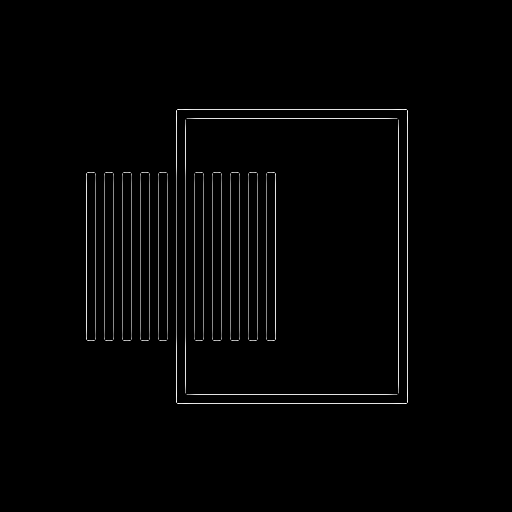
\includegraphics[width=.9\textwidth]{./canny/kanizsa_LINF_a4_k11_k24}
    \caption{kanizsa, Isotropic L-infinity norm. $\alpha$ = 4, K1 = 1, K2 = 4}
    \label{fig:kanizsa_LINF_a4_k11_k24}
  \end{subfigure}%

\end{figure}

\begin{figure}[H]
\centering

  \begin{subfigure}{.7\textwidth}
    \centering
    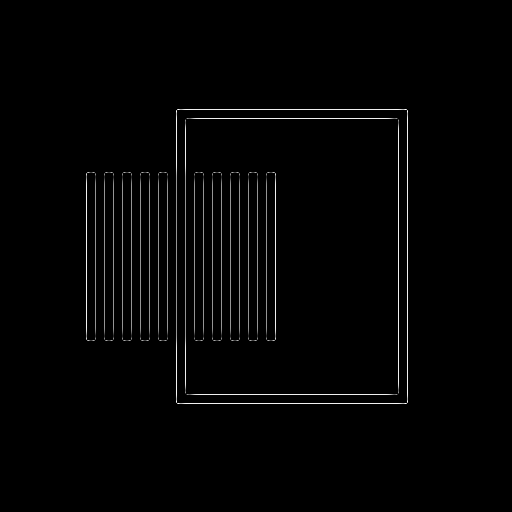
\includegraphics[width=.9\textwidth]{./canny/kanizsa_L1_a4_k11_k24}
    \caption{kanizsa, Isotropic L1 norm. $\alpha$ = 4, K1 = 1, K2 = 4}
    \label{fig:kanizsa_L1_a4_k11_k24}
  \end{subfigure}%
  
  \begin{subfigure}{.7\textwidth}
    \centering
    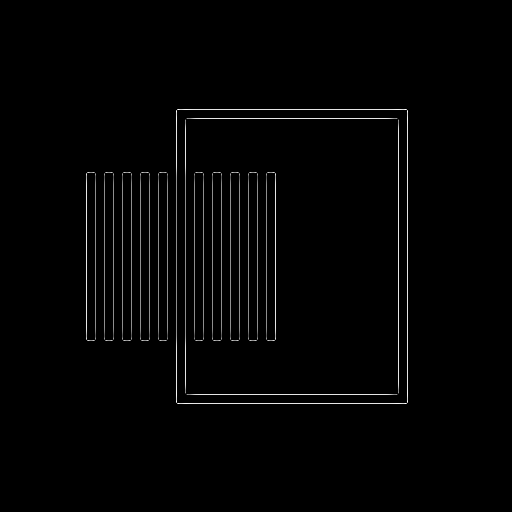
\includegraphics[width=.9\textwidth]{./canny/kanizsa_L2_a4_k11_k24}
    \caption{kanizsa, Isotropic L2 norm. $\alpha$ = 4, K1 = 1, K2 = 4}
    \label{fig:kanizsa_L2_a4_k11_k24}
  \end{subfigure}\\%
 \end{figure}

\begin{figure}[H]
\centering 
  \begin{subfigure}{.7\textwidth}
    \centering
    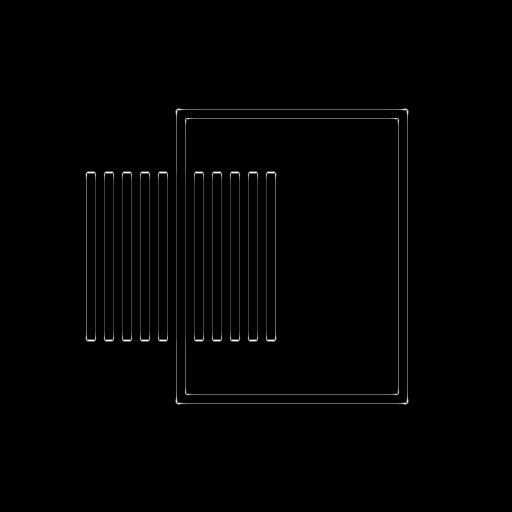
\includegraphics[width=.9\textwidth]{./canny/kanizsa_ANISO_a4_k11_k24}
    \caption{kanizsa, Anisotropic. $\alpha$ = 4, K1 = 1, K2 = 4}
    \label{fig:kanizsa_ANISO_a4_k11_k24}
  \end{subfigure}%
  
\end{figure}